\chapter{Evaluation and calibration of a new routing scheme over the Iberian Peninsula}
\label{chap:routing}
\minitoc
\pagebreak

\section{Chapter introduction}

This chapter presents the preliminary work to evaluate and calibrate the new version of the routing scheme (\native) before running coupled simulations with ICOLMDZOR. As a reminder, the pre-existing version of the routing scheme \std cannot be used with ICOLMDZOR because it imposes constraints on the ORCHIDEE and routing grids that are incompatible with the icosahedral grid. 
The \native routing is based on the same modelling principles (described in Chapter \ref{chap:methods}) as \std but relies on a new code to interpolate between the ORCHIDEE grid and the routing grid, and other changes to make it compatible with any DEM and ORCHIDEE grid.

Two objectives were initially identified:
\begin{itemize}
    \item Ensure that the \native code could generally replicate the behaviour of \std if given the same parameters and DEM as input. 
    \item Evaluate and calibrate \native using a high resolution DEM over the Iberian Peninsula to identify an appropriate set of parameters for coupled simulations.
\end{itemize}

However, this work raised more general scientific questions, which were partly addressed using offline simulations with different experimental setups. The routing modelling principles are theoretically independent of the spatial and temporal resolution but using \native allowed to look into the effects of changing to a high resolution DEM. During the calibration, which used discharge observations as a reference, the relative importance of various factors was also analysed, such as the meteorological forcing used and the activation of irrigation. It also raised the question of how the irrigation scheme could be adapted to better match regional practices and achieve more realistic values of river discharge in irrigated river basins. Finally, an important question was the impact and strength of the interdependency between irrigation, the water volume in the river reservoir and simulated river discharge in large basins.

\section{Methods for the routing scheme evaluation and calibration}

The relevant routing outputs for evaluation and calibration are river discharge and water volumes in each of the reservoirs (groundwater, overland, rivers). 
It must be noted that these volumes cannot be easily compared to observations, since large-scale measurements of groundwater or river volumes are complex and may not physically correspond to the abstraction level of the reservoirs modelled in ORCHIDEE.
Theie importance in this work is mainly justified by the fact that the irrigation scheme withdraws water from these reservoirs to satisfy the irrigation demand while conserving water quantities.

All simulations for this chapter were run in offline mode, meaning that ORCHIDEE is not coupled to any atmospheric model but takes meteorological data as input. 
Most simulations were run from 2000 to 2012, with the WATCH Forcing Data ERA-Interim \citep[WFDEI, ][]{weedon_wfdei_2014}. Sensitivity experiments to assess the impact of the forcing were also run with the Global Soil Wetness Project Phase 3 Atmospheric Boundary Conditions \citep[GSWP3, ][]{kim_hyungjun_global_2017}, another forcing dataset which is only available until 2010.
In all simulations, the first three years were considered as a spin-up and removed from the analysis, to allow the vegetation and hydrological variables to reach an equilibrium. The regional domain covers the Iberian Peninsula and part of Morocco, since at the time, this region was also considered as a study area for coupled simulations. Since this idea was not pursued, the analysis only focuses on the Iberian Peninsula.
Topographical data from the two DEMs presented in Chapter \ref{chap:methods} was used, either from the 0.5°-resolution DEM historically associated with the \std routing or from the MERIT DEM at 2-km resolution.

In all this chapter, the simulated river discharge is evaluated against monthly observation data from discharge stations of the Global Runoff Data Center \cite[GRDC, https://grdc.bafg.de,][]{fekete_global_2003}.
Stations were positioned on the 0.5° DEM grid using only the GPS position, and on the MERIT DEM grid with tools presented in \cite{polcher_hydrological_2023}, which use the GPS position of the stations as well as the upstream catchment area to find the most appropriate grid cell for comparison with the observations. 
Four stations were used, which are all on large rivers (Ebro, Douro, Tagus, Guadiana) and show large discharge values, meaning they represent the integrated discharge over a large share of the basins.

\begin{figure}[htbp]
    \centering
    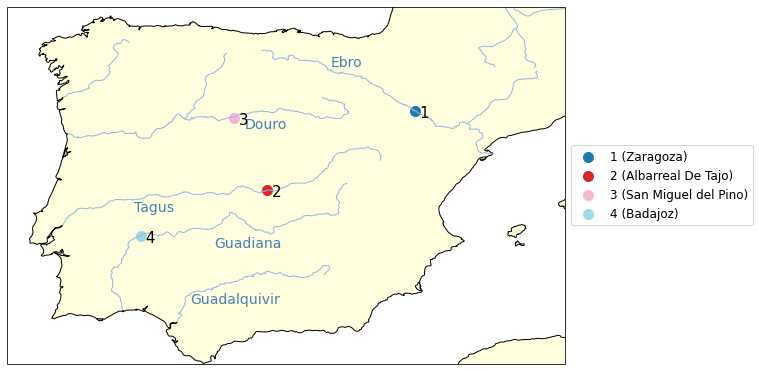
\includegraphics[width=0.7\textwidth]{images/chap3/river_discharge/halfdeg_4stations_map.png}
    \caption{Discharge stations selected for the routing scheme evaluation and calibration.}
    \label{fig:halfedg_stations_map}
\end{figure}

\section{Consistency of \native with \std routing}
\subsection{Simulation experiments}

This first analysis used the \native routing in the same setup as the \std routing. 
The input DEM was the same (0.5° resolution), and the time constants for the three reservoirs were the same as the default values for the global model (Table \ref{table:tcst_refs}).
Four simulations were run, two without irrigation (labeled as \textit{no\_irr}) to assess the routing schemes without its influence, and two with irrigation (labeled as \textit{irr}). It must be noted that these simulations were not aimed at evaluating the realism of simulated irrigation or discharge (which will be addressed in Section \ref{section:calib}) but only to assess if the new routing code behaves similarly to the previous version.

\begin{table}[h]
\centering
\begin{tabular}{|c|c|c|}
\hline
\textbf{TCST\_SLOW} & \textbf{TCST\_FAST} & \textbf{TCST\_STREAM} \\ \hline
25            & 3             & 0.24            \\ \hline
\end{tabular}
\caption{Routing time constant for the consistency analysis ($day \cdot km^{-1}$).}
\label{table:tcst_consistency}
\end{table}

\subsection{Results}

%figure : 12 maps of mean reservoir volumes and hydrographs, for both sims and diff
\begin{figure}[htbp]
    \centering
    \begin{tabular}{ccc}
        \begin{subfigure}[b]{0.33\textwidth}
            \caption{Groundwater reservoir\\(annual mean, \std)}
            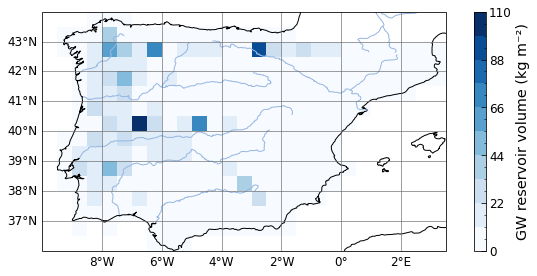
\includegraphics[width=\textwidth]{images/chap3/maps/slowr_subgrid.png}
        \end{subfigure} &
        \begin{subfigure}[b]{0.33\textwidth}
            \caption{Groundwater reservoir\\(annual mean, \native)}
            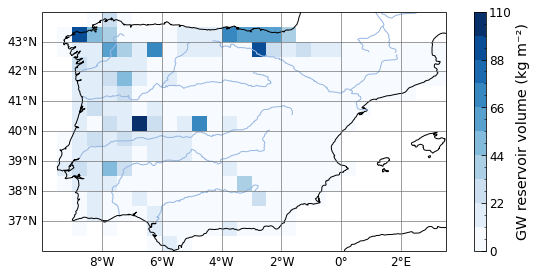
\includegraphics[width=\textwidth]{images/chap3/maps/slowr_interp.png}
        \end{subfigure} &
        \begin{subfigure}[b]{0.33\textwidth}
            \caption{Groundwater reservoir (difference, \native - \std)}
            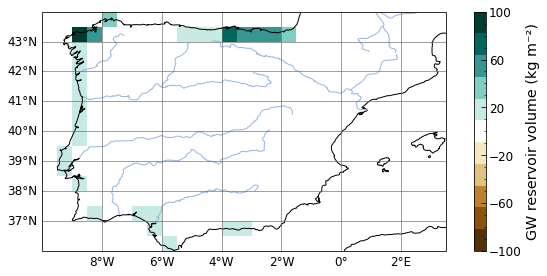
\includegraphics[width=\textwidth]{images/chap3/maps/slowr_diff.png}
        \end{subfigure} \\
        
        \begin{subfigure}[b]{0.33\textwidth}
            \caption{Surface water reservoir\\(annual mean, \std)}
            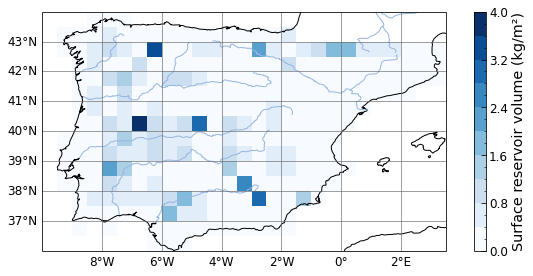
\includegraphics[width=\textwidth]{images/chap3/maps/fastr_subgrid.png}
        \end{subfigure} &
        \begin{subfigure}[b]{0.33\textwidth}
            \caption{Surface water reservoir\\(annual mean, \native)}
            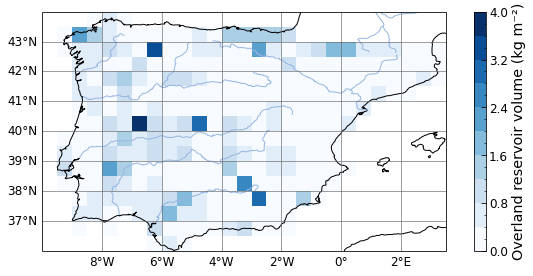
\includegraphics[width=\textwidth]{images/chap3/maps/fastr_interp.png}
        \end{subfigure} &
        \begin{subfigure}[b]{0.33\textwidth}
            \caption{Surface water reservoir (difference, \native - \std)}
            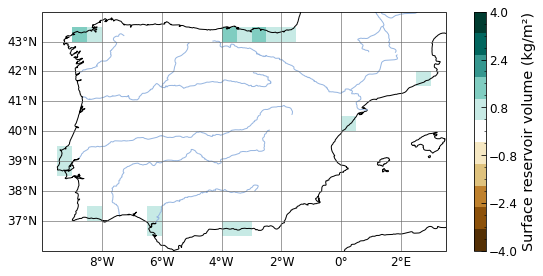
\includegraphics[width=\textwidth]{images/chap3/maps/fastr_diff.png}
        \end{subfigure} \\
        
        \begin{subfigure}[b]{0.33\textwidth}
            \caption{River reservoir\\(annual mean, \std)}
            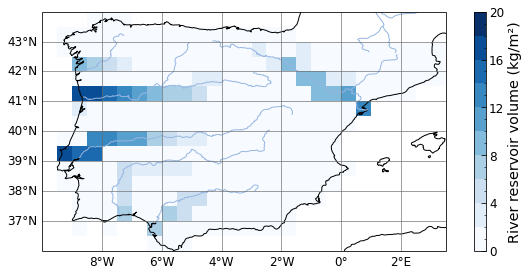
\includegraphics[width=\textwidth]{images/chap3/maps/streamr_subgrid.png}
        \end{subfigure} &
        \begin{subfigure}[b]{0.33\textwidth}
            \caption{River reservoir\\(annual mean, \native)}
            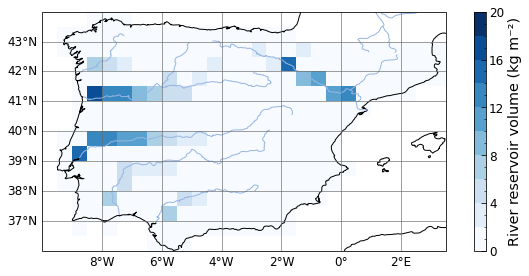
\includegraphics[width=\textwidth]{images/chap3/maps/streamr_interp.png}
        \end{subfigure} &
        \begin{subfigure}[b]{0.33\textwidth}
            \caption{River reservoir (difference, \native - \std)}
            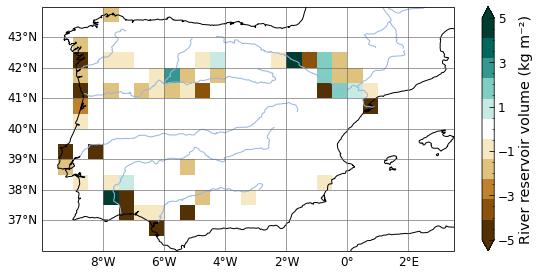
\includegraphics[width=\textwidth]{images/chap3/maps/streamr_diff.png}
        \end{subfigure} \\
        
        \begin{subfigure}[b]{0.33\textwidth}
            \caption{River discharge\\(annual mean, \std)}
            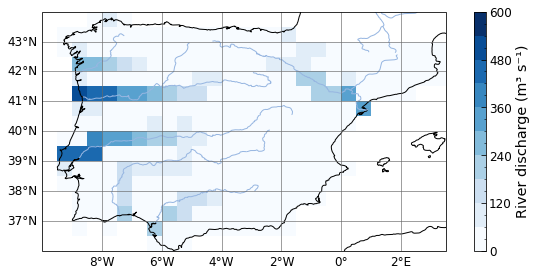
\includegraphics[width=\textwidth]{images/chap3/maps/hydrographs_subgrid.png}
        \end{subfigure} &
        \begin{subfigure}[b]{0.33\textwidth}
            \caption{River discharge\\(annual mean, \native)}
            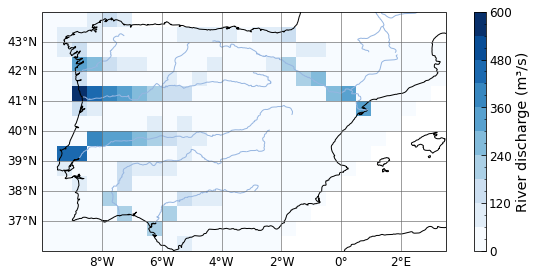
\includegraphics[width=\textwidth]{images/chap3/maps/hydrographs_interp.png}
        \end{subfigure} &
        \begin{subfigure}[b]{0.33\textwidth}
            \caption{River discharge (difference, \native - \std)}
            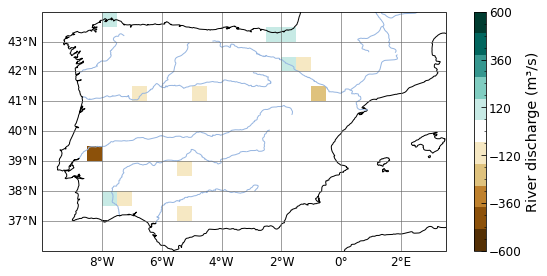
\includegraphics[width=\textwidth]{images/chap3/maps/hydrographs_diff.png}
        \end{subfigure} \\
    \end{tabular}
    \caption{Annual mean (2003-2012) of reservoir volumes and river discharge for \std (\noirr), \native (\noirr) and difference between them. 
    Although this is not the case for reservoir variables, the scale for (l) was deliberately chosen much smaller than (j) and (k) to highlight differences between the two simulations.}
    \label{fig:routing_reservoirs_halfdeg}
\end{figure}

The comparison of the mean volumes for the groundwater and overland reservoirs (Fig. \ref{fig:routing_reservoirs_halfdeg}a-f) shows differences only on coastal grid cells, which are very low in \std but can have significant values in \native. This is particularly visible in the northern moutain ranges, and it must be noted that the values computed by \native are in the expected order of magnitude, considering these are regions of high precipitation, and therefore high drainage and surface runoff.
These differences are thought to be the consequence of a different handling of water quantities and their units in \native compared to \std. Drainage and surface runoff are computed on the ORCHIDEE grid, in $kg m^{-2}$ (equivalent to $mm$ over the grid cell) and in \native, they are  converted to absolute water quantities (in $kg$) before being interpolated to the DEM grid. These absolute quantities are routed on the DEM grid and the new water quantities in the reservoirs are reinterpolated to the ORCHIDEE grid (even when the two grids have the same resolution). 
To express them as an areal value, in $kg m^{-2}$, the absolute water quantity has to be divided by the area of the grid cell. It is considered likely that this back-and-forth interpolation and change of units introduces the differences, by accounting for continental fraction (to obtain the exact area on coastal points) whereas in \std this was not necessary since all computations were on the same grid cell. Such subtleties in the code were introduced to enable compatibility with any DEM grid and are still under investigation by its developpers to clarify the cause of the observed discrepancies and determine whether they introduced errors or corrected existing flaws of the previous code.
Since this issue affected only the groundwater and overland reservoirs and was located only on coastal grid cells, it was considered that for the purpose of this thesis, the impacts should not affect the results substantially and that \native could be used in its current version.
%todo:continuer à clarifier avec Antoine et/ou Yann pour mieux expliquer ? 

Regarding the stream reservoir (Fig. \ref{fig:routing_reservoirs_halfdeg}g-i), a new modelling choice was made on coastal grid cells. In \std, there was a stream reservoir for these grid cells, whereas it was removed in \native. This choice was made during the development of the scheme and might be changed in future versions to ensure consistency with the other two reservoirs. 
The way to compute river discharge (m³/s) in these coastal points is also slightly different in \native, as it includes the flow from the stream reservoir of the upstream grid cell, as well as the flow from the groundwater and overland reservoirs of the grid cell, whereas drainage and surface runoff were considered to flow directly in the ocean in \std. This explains why discharge values are or similar order of magnitude but larger in \native (Fig. \ref{fig:routing_reservoirs_halfdeg}l). 
Figure \ref{fig:coastal_routing_behaviour} schematizes the differences in implementation that explain the differences seen in the river reservoir and in the discharge on coastal grid cells.

\begin{figure}[htbp]
    \centering
    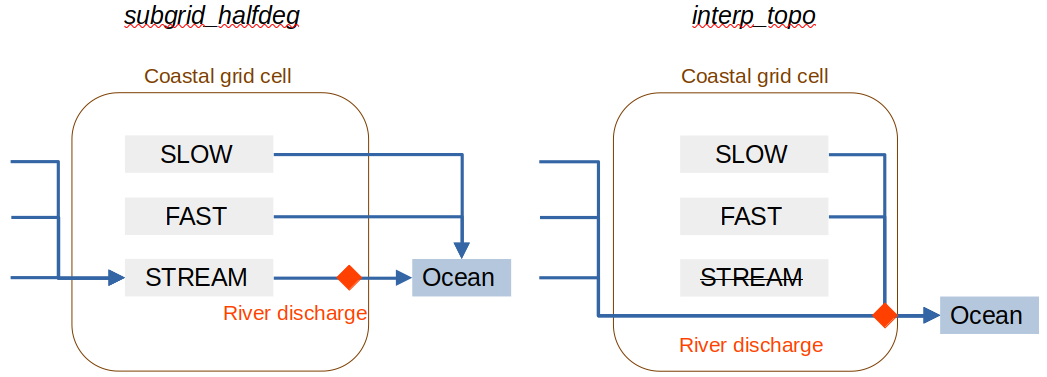
\includegraphics[width=\textwidth]{images/chap3/coastal_routing_behaviour_v2.png
}
    \caption{Differences in implementation between \std and \native on coastal grid cells.}
    \label{fig:coastal_routing_behaviour}
\end{figure}

Appart from coastal grid cell, the most noticeable discrepancy on the stream reservoir and river discharge is that some non-coastal points have different values in both routing versions. It can be seen on Fig. \ref{fig:routing_reservoirs_halfdeg}j-l particularly that the water does not flow exactly in the same path, meaning that the DEM is not interpreted exactly in the same way. This has been attributed to preprocessings of the DEM implemented in \std to avoid creating dead-ends, grid cells where the water would not keep flowing and accumulate in the stream reservoir. These changes in the routing graph were implemented when developing the routing scheme for global applications, possibly with a focus on other ORCHIDEE grid resolutions (1° or 2° instead of the 0.5° used here) and do not seem necessary when routing water directly on the DEM, which is why they were not implemented in \native. In the large rivers where there are differences, \native seems to use shorter paths that \std, often flowing diagonally to the next grid cell instead of taking two 90° turns. In most of the domain, on annual average, this seems to lead to smaller amounts of water in the river reservoir and smaller discharge in \native compared to \std, as clearly visible on the Duero river in Fig. \ref{fig:routing_reservoirs_halfdeg}l.

%figure : 3 time series (3 reservoirs)on average over the IP for both routings
\begin{figure}[htbp]
    \centering
    \begin{subfigure}[b]{0.32\textwidth}
        \caption{Groundwater reservoir average}
        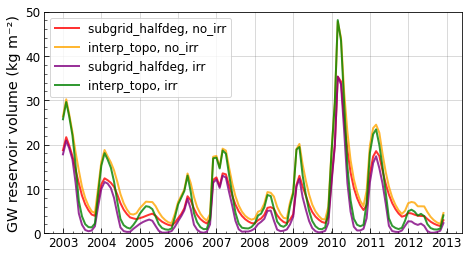
\includegraphics[width=\textwidth]{images/chap3/time_series/slowr_time_series.png}
    \end{subfigure}
    \begin{subfigure}[b]{0.32\textwidth}
        \caption{Surface water reservoir average}
        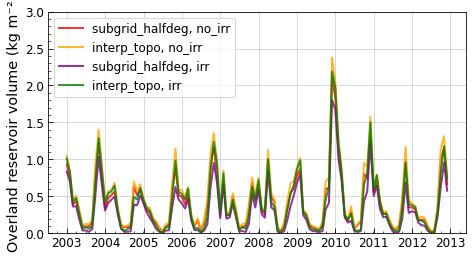
\includegraphics[width=\textwidth]{images/chap3/time_series/fastr_time_series.png}
    \end{subfigure}
    \begin{subfigure}[b]{0.32\textwidth}
        \caption{River reservoir average}
        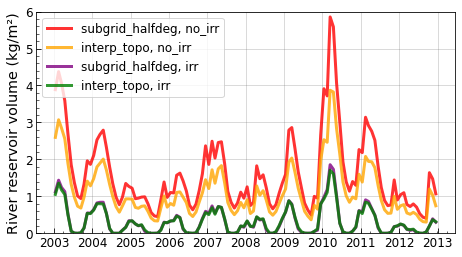
\includegraphics[width=\textwidth]{images/chap3/time_series/streamr_time_series.png}
    \end{subfigure} \\

    \begin{subfigure}[b]{0.32\textwidth}
        \caption{Groundwater reservoir average seasonal cycle}
        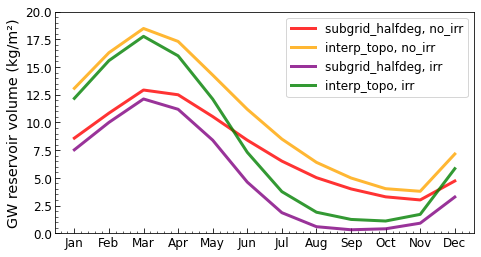
\includegraphics[width=\textwidth]{images/chap3/time_series/slowr_seasonal_cycle.png}
    \end{subfigure}
    \begin{subfigure}[b]{0.32\textwidth}
        \caption{Surface water reservoir average seasonal cycle}
        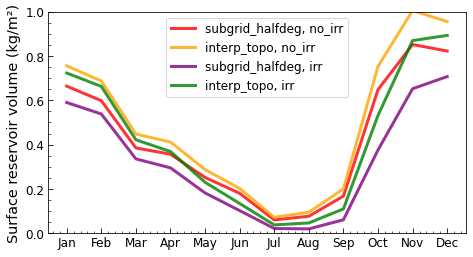
\includegraphics[width=\textwidth]{images/chap3/time_series/fastr_seasonal_cycle.png}
    \end{subfigure}
    \begin{subfigure}[b]{0.32\textwidth}
        \caption{River reservoir average seasonal cycle}
        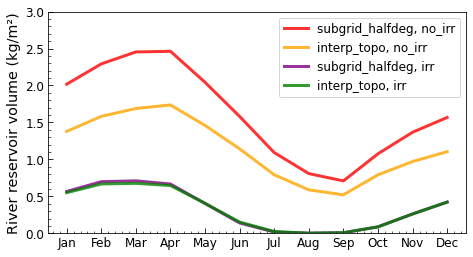
\includegraphics[width=\textwidth]{images/chap3/time_series/streamr_seasonal_cycle.png}
    \end{subfigure}
    \caption{Time series and seasonal cycles of reservoir volumes on average over the Iberian Peninsula domain.}
    \label{fig:reservoir_time_series}
\end{figure}

On average over the Peninsula, the differences noticed above are visible in the groundwater and overland reservoirs where \native has larger volumes due to water in coastal grid cells (Fig. \ref{fig:reservoir_time_series}a, b). On the river reservoir however, \std has larger volumes, mostly due to the absence of this reservoir on coastal points with river outlets, which are the grid cells with the largest volumes in \std.
If all coastal grid cells were to be removed from the average (not shown)%option: faire la figure ? ou annexe ?
, there would be no difference on the groundwater and overland reservoirs, and a much difference on the river reservoir, although \std still has more water stored in this reservoir than \native, particularly in winter and spring, when there is more rain in the region. This confirms the previous observation that water follows shorter paths to the sea in \native and therefore, does not remain in the river reservoir as long as in \std.
In the \irr simulations (purple and green lines in Fig. \ref{fig:reservoir_time_series}), all reservoirs are partly depleted by the irrigation withdrawals. For the groundwater and overland reservoirs, the differences between \std and \native mostly remain, since they are located in coastal grid cells, which are seldom intensely irrigated.
Regarding the river reservoir (Fig. \ref{fig:reservoir_time_series}f), \std simulates much lower volumes in the \irr than in \noirr simulation (-75\% in winter and complete depletion in summer). This decrease is also seen with \native, and the differences between the two routing versions almost disappear. This is consistent with the source of these differences, since the \irr simulations simulate much lower volumes in rivers, the discrepancies in the routing graph and at the river outlets have much less impact on the average volume over the domain.

%figure : 3 maps of simulated irrigation (subgrid, interp, diff), TS and SC of irrig for both simulations
\begin{figure}[htbp]
    \centering
    \begin{subfigure}[b]{0.32\textwidth}
        \caption{Irrigation annual mean\\(\std)}
        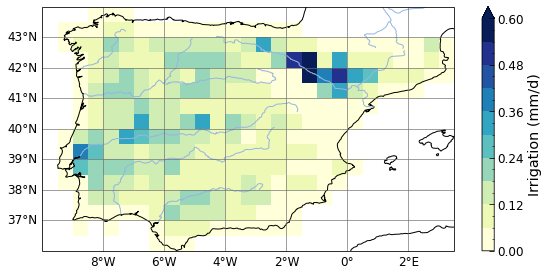
\includegraphics[width=\textwidth]{images/chap3/maps/irrigation_subgrid.png}
    \end{subfigure}
    \begin{subfigure}[b]{0.32\textwidth}
        \caption{Irrigation annual mean\\(\native)}
        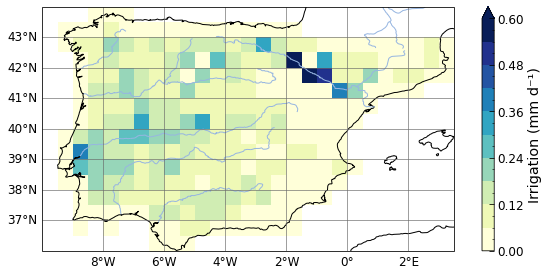
\includegraphics[width=\textwidth]{images/chap3/maps/irrigation_interp.png}
    \end{subfigure}
    \begin{subfigure}[b]{0.32\textwidth}
        \caption{Irrigation difference\\(\native - \std)}
        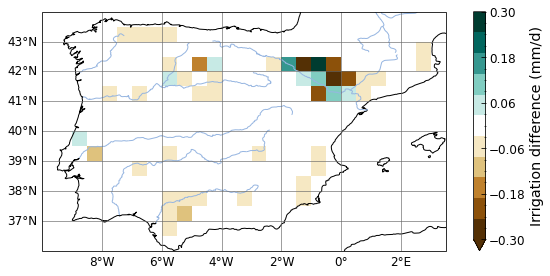
\includegraphics[width=\textwidth]{images/chap3/maps/irrigation_diff.png}
    \end{subfigure} \\

    \begin{subfigure}[b]{0.48\textwidth}
        \caption{Irrigation (Iberian Peninsula average)}
        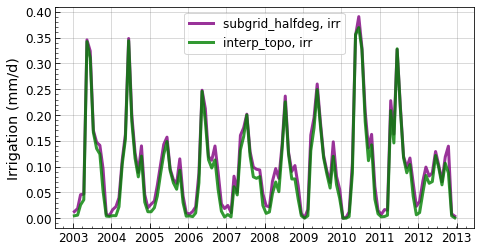
\includegraphics[width=\textwidth]{images/chap3/time_series/irrigation_time_series.png}
    \end{subfigure}    
    \begin{subfigure}[b]{0.48\textwidth}
        \caption{Irrigation average seasonal cycle}
        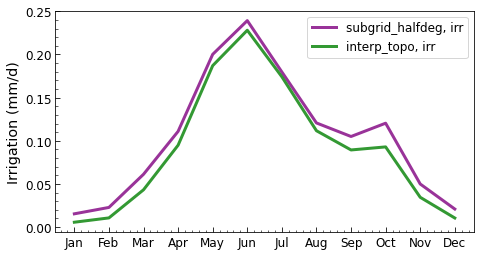
\includegraphics[width=\textwidth]{images/chap3/time_series/irrigation_seasonal_cycle.png}
    \end{subfigure}

    \caption{Simulated irrigation in \std and \native. Annual mean for both simulations (a,b) and difference (c). Average time series (d) and seasonal cycle (e) over the Iberian Peninsula.}
    \label{fig:irrigation_halfdeg_eval}
\end{figure}

Both simulations show a similar simulated irrigation (Fig. \ref{fig:irrigation_halfdeg_eval}a, b), but the differences on reservoir volumes affect the available water, and therefore irrigation. This is particlarly visible in the Ebro valley where some grid cells are highly irrigated in one simulation and not in the other. This is due to the aforementionned differences in the routing graph, which affect the path of the Ebro river (Fig. \ref{fig:irrigation_halfdeg_eval}c), the main source for irrigation withdrawals in the region.
On average over the domain (Fig. \ref{fig:irrigation_halfdeg_eval}d, e) \std exhibits slightly higher volumes of irrigation than \native, which is consistent with the higher volumes in the river reservoir. As previously explained, the differences seen in the reservoirs on coastal grid cells seem to have little impacts on the irrigated volumes, since these regions are seldom intensely irrigated. %todo:ref to irrigmap figure ? In methods ?
%todo: comment more on depletion, irrigation limited by available water, and second peak in autumn which is enabled by new rain

%figure : river discharge seasonal cycle for 4 stations (large rivers but not Guadalquivir...), 2 routing versions, irr and no_irr for each
\begin{figure}[htbp]
    \centering
    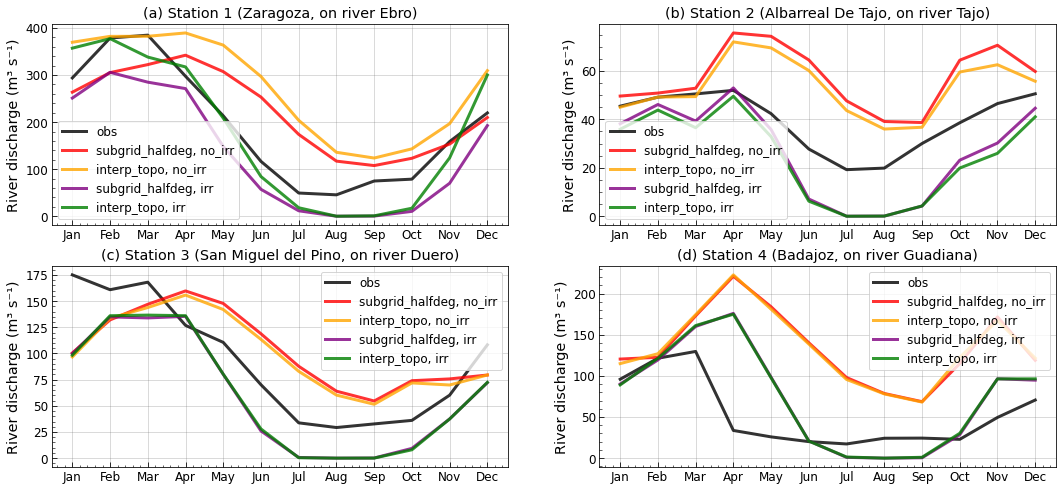
\includegraphics[width=\textwidth]{images/chap3/river_discharge/halfdeg_4stations_SC.png}
    \caption{River discharge mean seasonal cycle (2003-2012) for 4 large stations of the Peninsula.}
    \label{fig:halfdeg_stations_SC}
\end{figure}

The seasonal cycle of river discharge reflects the general agreement of the two routing versions, without irrigation, the red and yellow lines follow each other closely, and with irrigation, the purple and green are also very similar. Some differences persist, due to the differences in the routing graph already described, mostly for the Ebro river since the station is downstream of several discrepancies visible on Fig. \ref{fig:routing_reservoirs_halfdeg}l.

\subsection{Conclusions}

This comparison of the \native routing version with \std showed that this new version is generally reproducing the modelling principles correctly, but several differences were identified between the two versions. All three reservoirs are handled differently in \native on coastal grid cells, which affects the average volumes stored over the Iberian Peninsula, but does not have a significant impact on irrigation or river dicharge. However, differences in the path followed by water as it flows from one grid cell to another in the river reservoirs are also clearly identified in large rivers of the Peninsula. This leads to local changes in the simulated river dicharge, and slightly less water stored in the river reservoir by \native since it simulated shorter paths in several occurrences. These discrepancies also have an impact on irrigation since it is strongly reliant on the volumes of water available in the river reservoir, but this impact remains limited on average over the domain.

\section{Calibration over the Iberian Peninsula}
\label{section:calib}

Once the general consistency of the \native routing had been assessed, it became possible to evaluate the specific setup that would be used for the coupled simulation, using the MERIT DEM at 2km resolution and accounting for irrigation. To use irrigation, the routing time step must be the same as the time step of ORCHIDEE, which is 15mn (900s) in coupled simulations. 

This calibration was initially focused on the three time constants of the routing reservoirs: TCST\_SLOW, TCST\_FAST, TCST\_STREAM. Although these parameters should theoretically be independent of the spatial and temporal time steps and of the DEM used as input, they can strongly influence the results. %todo : rephrase
In particular, the ORCHIDEE routing scheme had never been used with a high-resolution topography like the MERIT DEM at 2-km resolution, since the \std routing ran only with the 0.5° resolution DEM used in the previous section, and often with a 24-hours routing time step. Multiple tests were therefore carried to identify an appopriate set of time constants for the reservoirs.
Moreover, the sensitivity of river discharge to the activation of irrigation was identified as very important, with large differences in the responses depending on the intensity of irrigation demand. As a consequence, the parameter $\beta$, which defines the soil moisture target in the irrigation scheme, was also included in this calibration and modified compared to the default version of the model.

\subsection{Simulation experiments}

At the begining of the calibration, three reference sets of TCST parameters (presented in Table \ref{table:tcst_refs}) were considered:
\begin{itemize}
\item The values established during an initial calibration of the \native routing performed over the Danube basin, which focused only on river discharge observations \citep{kilic_evaluation_2023}.
\item The default values used by the \std routing on a global scale, which were used in the previous section with the 0.5° DEM. These values were identified empirically by a calibration study over the Senegal river basin and validated globally in \citet{ngo-duc_53-year_2005, ngo-duc_validation_2007} using river discharge and groundwater measurements from Gravity Recovery and Climate Experiment (GRACE) satellite data.
\item The values used for regional studies with the \textit{subgrid\_HTU} routing \citep{rinchiuso_improving_2022, huang_multi-objective_2024}.
\end{itemize}

\begin{table}[h]
\centering
\begin{tabular}{|l|c|c|c|}
\hline
\textbf{} & \textbf{TCST\_SLOW} & \textbf{TCST\_FAST} & \textbf{TCST\_STREAM} \\ \hline
Initial \native calibration & 1.2 & 0.9 & 0.03 \\ \hline
\std default values & 25 & 3 & 0.24 \\ \hline
\textit{Subgrid\_HTU} calibration & 600 & 80 & 6.3 \\ \hline
\end{tabular}
\caption{Reference parameter sets considered to calibrate the \native routing ($day \cdot km^{-1}$).}
\label{table:tcst_refs}
\end{table}

In these three sets of values, there is approximately an order of magnitude between the three time constants, and very significant differences (one or two orders of magnitude) between each set. 
This can be explained by the different DEMs used, the way HTUs are defined, and the calibration choices that led to these sets of values.%option:compléter explication ? 

Three initial experiments were defined, based on these ratios:\\$TCST\_SLOW \approx 10 \times TCST\_FAST \approx 100 \times TCST\_STREAM$.
Table \ref{table:tcst_exp} presents these three sets of values based on the orders of magnitude of each of the reference value sets (TCST1, TCST2, TCST3), as well as the one selected after the calibration (TCST4), whose development steps are detailed hereafter.

\begin{table}[h]
\centering
\begin{tabular}{|l|c|c|c|}
\hline
\textbf{} & \textbf{TCST\_SLOW} & \textbf{TCST\_FAST} & \textbf{TCST\_STREAM} \\ \hline
TCST1 & 3 & 0.3 & 0.03 \\ \hline
TCST2 & 30 & 3 & 0.3 \\ \hline
TCST3 & 300 & 30 & 3 \\ \hline
TCST4 & 700 & 100 & 0.1 \\ \hline
\end{tabular}
\caption{Value sets of the simulations for the calibration of the \native routing ($day \cdot km^{-1}$).}
\label{table:tcst_exp}
\end{table}

Four simulations without irrigation were therefore carried out with these four sets of TCST values over the period 2000-2012 and analysed over 2003-2012.

\subsection{Reservoir volumes and time constants}

Volumes in each of the reservoirs were first compared to the volumes simulated by the \std routing. As a reminder, this version, with the 0.5° DEM, has long been used in ORCHIDEE and was evaluated against groundwater reference products from GRACE, as well as river discharge observations  \citep{ngo-duc_53-year_2005, ngo-duc_validation_2007}.
It is also the version that was used for the evaluation and validation of the irrigation scheme at global scale \citep{arboleda-obando_validation_2024}, which makes it a relevant reference for the reservoir volumes since available water is a major driver of simulated irrigation in the model. 

On average over the Peninsula, for the groundwater and surface water reservoirs, the TCST3 simulation showed values closest to \std (Fig. \ref{fig:reservoir_time_series_tcsts}a, b, d, e), while TCST1 and TCST2 hold almost no water in these reservoirs, meaning that they flow more quickly in the river reservoir. On the river reservoir however (Fig. \ref{fig:reservoir_time_series_tcsts}c, f), TCST3 is one order of magnitude above the other simulation, including \std, hinting that the value to TCST\_STREAM is too large for this reservoir, meaning that water circulates too slowly. This is confirmed looking at river discharge (Fig. \ref{fig:merit_tcsts_stations_SC}), as TCST3 cannot reproduce the observed structure of the seasonal cycle for any of the four rivers considered. These results, as well as a few intermediate tests not shown here, led to the choice of a new set of parameters (TCST4), which has values similar to TCST3 for the groundwater and overland reservoirs, but closer to TCST2 (even slightly faster) for the river reservoir (\ref{table:tcst_exp}), shown in red in Fig. \ref{fig:reservoir_time_series_tcsts} and \ref{fig:merit_tcsts_stations_SC}.
Average simulated volumes for TCST4 are clos to \std on all reservoirs, and match discharge observations with similar performance to TCST1 and TCST2.
%todo:add metrics ? KGE, BIAS

It can be noted that the performance of TCST1 for river dischage is good, but that it holds almost no water in the groundwater and overland reservoirs, suggesting that this previous calibration with the 2-km MERIT DEM focusing only on matching discharge observations \citep{kilic_evaluation_2023} neglected some aspects of the routing scheme and effectively calibrated only TCST\_STREAM.


%figure : 3 time series (3 reservoirs) on average over the IP for 4 tcsts and std as reference
\begin{figure}[htbp]
    \centering
    \begin{subfigure}[b]{0.32\textwidth}
        \caption{Groundwater reservoir average}
        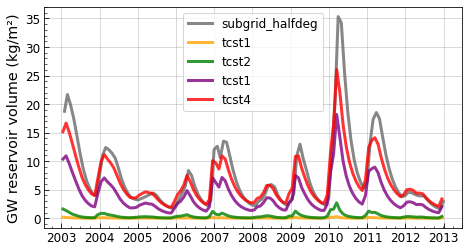
\includegraphics[width=\textwidth]{images/chap3/time_series/slowr_time_series_tcsts.png}
    \end{subfigure}
    \begin{subfigure}[b]{0.32\textwidth}
        \caption{Surface water average}
        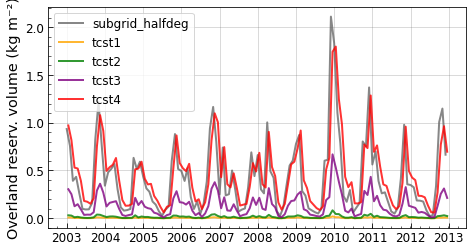
\includegraphics[width=\textwidth]{images/chap3/time_series/fastr_time_series_tcsts.png}
    \end{subfigure}
    \begin{subfigure}[b]{0.32\textwidth}
        \caption{River reservoir average}
        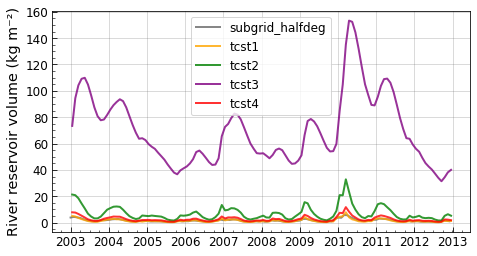
\includegraphics[width=\textwidth]{images/chap3/time_series/streamr_time_series_tcsts.png}
    \end{subfigure} \\

    \begin{subfigure}[b]{0.32\textwidth}
        \caption{Groundwater reservoir average seasonal cycle}
        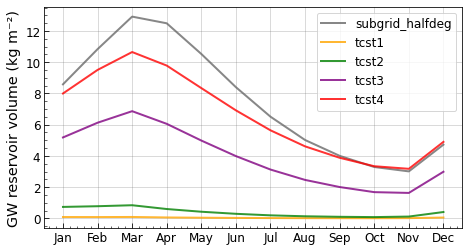
\includegraphics[width=\textwidth]{images/chap3/time_series/slowr_seasonal_cycle_tcsts.png}
    \end{subfigure}
    \begin{subfigure}[b]{0.32\textwidth}
        \caption{Surface water reservoir average seasonal cycle}
        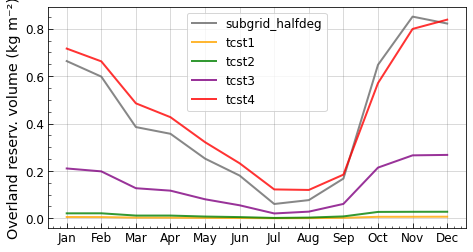
\includegraphics[width=\textwidth]{images/chap3/time_series/fastr_seasonal_cycle_tcsts.png}
    \end{subfigure}
    \begin{subfigure}[b]{0.32\textwidth}
        \caption{River reservoir average seasonal cycle}
        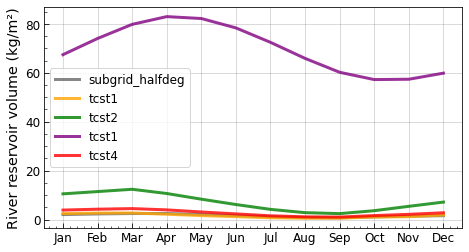
\includegraphics[width=\textwidth]{images/chap3/time_series/streamr_seasonal_cycle_tcsts.png}
    \end{subfigure}
    \caption{Time series and seasonal cycles of reservoir volumes on average over the Iberian Peninsula domain.}
    \label{fig:reservoir_time_series_tcsts}
\end{figure}

%figure : river discharge seasonal cycle for 4 stations (large rivers but not Guadalquivir...), 2 routing versions, irr and no_irr for each
\begin{figure}[htbp]
    \centering
    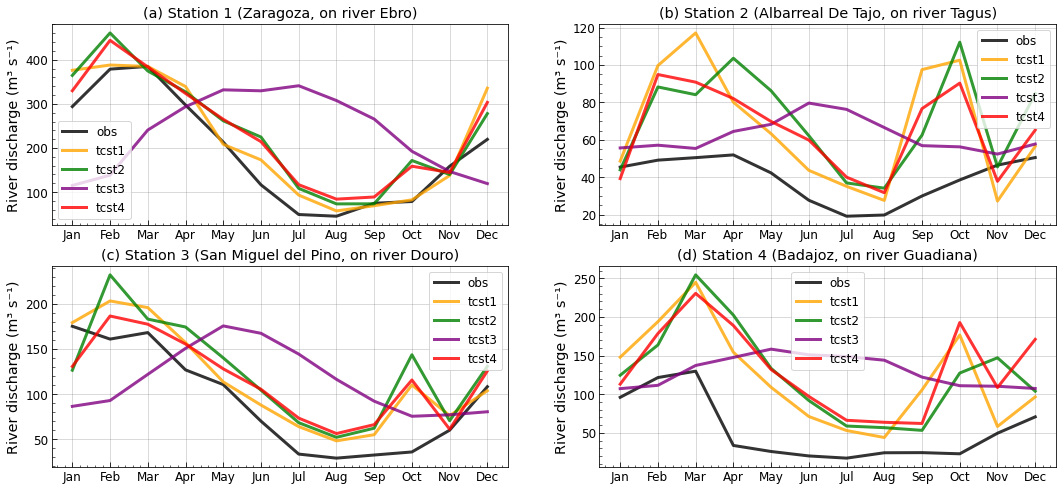
\includegraphics[width=\textwidth]{images/chap3/river_discharge/merit_tcst_4stations_SC.png}
    \caption{River discharge mean seasonal cycle (2003-2012) with four sets of TCST parameters.}
    \label{fig:merit_tcsts_stations_SC}
\end{figure}

Further tests for the choice of parameters were considered, to explore if the performance of the \native routing with MERIT DEM could be further improved regarding river discharge, but sensitivity experiments were first conducted, using the TCST4 parameter set, to assess the relevance of a finer tuning of the TCST parameters.

\subsection{Impacts of atmospheric forcing and irrigation on river discharge}

\begin{figure}[htbp]
    \centering
    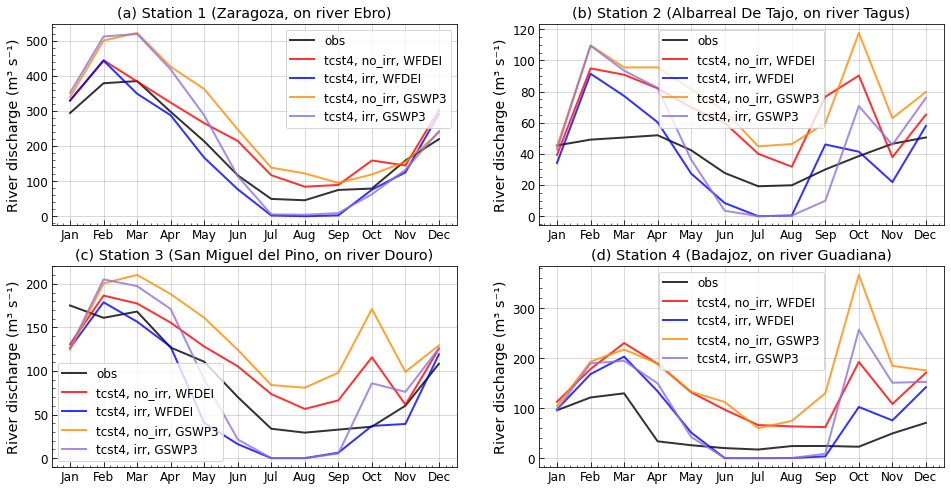
\includegraphics[width=\textwidth]{images/chap3/river_discharge/merit_forcing_4stations_SC.png}
    \caption{River discharge mean seasonal cycle (2003-2012) with GSWP3 and WFDEI forcings, with ant without irrigation.}
    \label{fig:merit_forcing_stations_SC}
\end{figure}

The impacts of the atmospheric forcing used and of irrigation were assessed jointly with four simulations, all with the TCST4 parameter set, using two atmospheric forcings (WFDEI and GSWP3), each with and without irrigation. Considering the availability of GSWP3, simulations were only run until 2010.

The results (Fig. \ref{fig:merit_forcing_stations_SC}) show a response to both changes but a stronger impact of irrigation, which strongly reduces discharge, except in winter. The WFDEI and GSWP3 forcing produce seasonal cycles with similar structures but using the GSWP3 forcing leads to larger discharge in the winter peak for the Ebro and Douro basin, as well in the peak of autumn precipitation in the Tagus, Douro and Guadiana basins. These regional and sesonal specificities reflect the differences in precipitation between the two forcings. %todo:show yearly or seasonal maps ? side by side, diff ?
In summer, the \noirr and \irr simulations with the two forcings are similar, especially with irrigation, which depletes the river reservoir, reducing discharge to near-zero for the four rivers.

The strengths of these responses, compared to the differences in the parameter sets explored in Fig. \ref{fig:merit_tcsts_stations_SC} justified the decision not to pursue finer tuning of the TCST parameters, which would be too dependent on the forcing or the activation of irrigation. The TCST4 parameter set was considered an acceptable option for the routing scheme, and it was decided to include the parameterization of irrigation in the calibration. 

\begin{figure}[htbp]
    \centering
    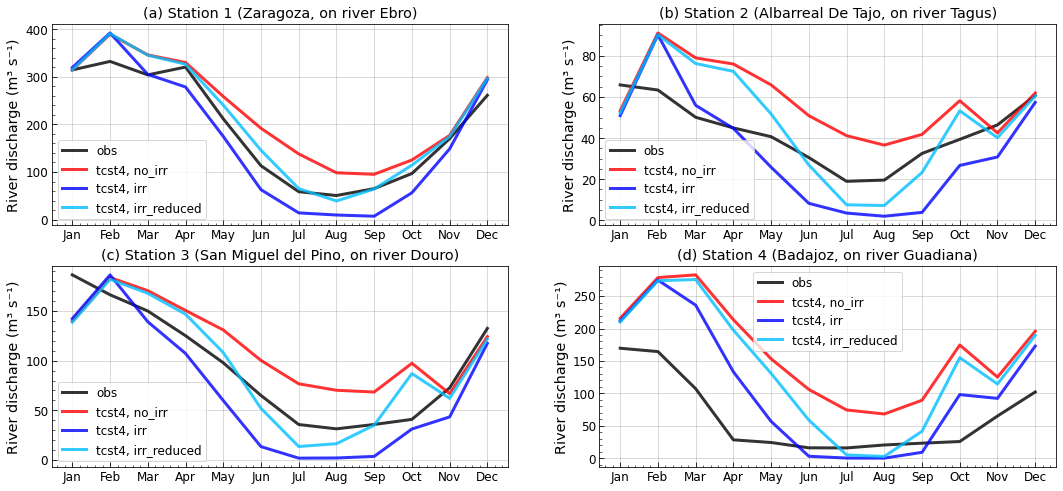
\includegraphics[width=\textwidth]{images/chap3/river_discharge/merit_irr_4stations_SC.png}
    \caption{River discharge mean seasonal cycle (2003-2010) in the \noirr, \irr and \textit{irr\_reduced} simulations.}
    \label{fig:merit_irr_stations_SC}
\end{figure}

The global evaluation of the ORCHIDEE irrigation scheme \citep{arboleda-obando_validation_2024} identified the \betairrig parameter as the main driver of simulated irrigation. This parameter conditions the soil moisture target as a fraction of soil moisture at field capacity. The default value selected for global simulations was \betairrig = 0.9. However, this value was chosen as an average on the global scale, meant to reflect a large diversity of irrigation practices, including flooding methods in rice paddies, which is common in intensely irrigated regions of northern India and China. For such practices, \betairrig = 1.2 would be more appropriate to represent the irrigation withdrawals properly. In the Iberian Peninsula however, the limited water supply and semiarid climate favor less water intensive methods (drip or sprinkler irrigation) which would be better represented with lower values of \betairrig. The value of $0.9$ was selected as a way to center the global biases compared to reference products on zero, acknowledging that this value was too low for some regions and too high for others.

This is why other values were explored for the calibration over the Iberian Peninsula, as well as to limit the unrealistic depletion of rivers in summer. Fig. \ref{fig:merit_irr_stations_SC} shows three simulations, all with the WFDEI forcing and TCST4 set of parameter for routing, but with different options for irrigation: \noirr, \irr (default value \betairrig = 0.9) and \textit{irr\_reduced} with \betairrig = 0.6. 
This simulation limits the depletion in summer and yields much better performance in the Ebro basin, which is the most very intensely irrigated region, and largely depends on water from river (as opposed to groundwater) for irrigation.
This reduced irrigation also seems more consistent when looking at the seasonal cycle of irrigation (Fig. \ref{fig:merit_irr_reduced}c). In the default \irr simulation, high volumes are withdrawn in the spring but irrigation drops in summer, which is the season where irrigation demand is the highest. This is due to a lack of available water in the reservoirs in the irrigated regions in summer, which are depleted too quickly when using \betairrig = 0.9. The effect of the river reservoir depletion is also visible on the summer river discharge of Fig. \ref{fig:merit_irr_stations_SC} which falls to near-zero for the four rivers considered.

To summarize, the \textit{irr\_reduced} setup simulates a lower demand in irriation and therefore less irrigation overall, but it avoids an early depletion of the reservoirs, yielding a more consistent seasonal cycle of irrigation and matching discharge observation better in spring and summer.
%option : also show root_deficit to demonstrate that large Beta leads to much larger demand

%figure : maps of irrig in irr and irr_reduced, and seasonal cycle of irrig over IP for both sims
\begin{figure}[htbp]
    \centering
    \begin{subfigure}[b]{0.32\textwidth}
        \caption{Mean irrigation in \irr.\\ } 
        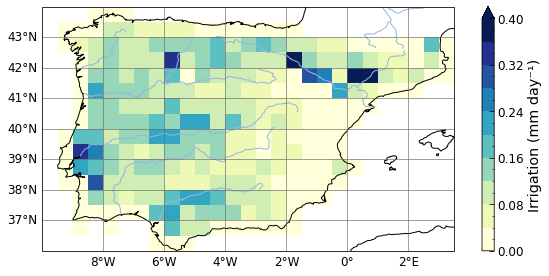
\includegraphics[width=\textwidth]{images/chap3/maps/irrigation_ave_tcst4_irr.png}
    \end{subfigure}
    \begin{subfigure}[b]{0.32\textwidth}
        \caption{Mean irrigation in \textit{irr\_reduced}.} 
        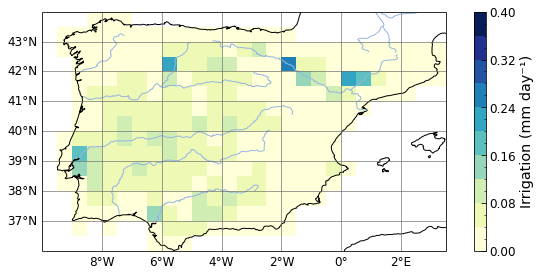
\includegraphics[width=\textwidth]{images/chap3/maps/irrigation_ave_tcst4_irr_reduced.png}
    \end{subfigure}
    \begin{subfigure}[b]{0.32\textwidth}        
        \caption{Seasonnal cycle of irrigation.} 
        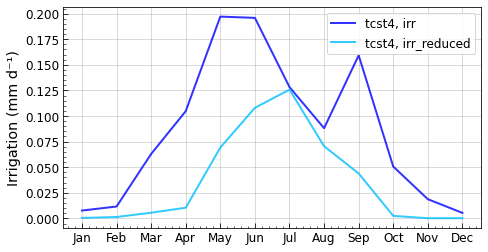
\includegraphics[width=\textwidth]{images/chap3/time_series/irrigation_seasonal_cycle_irr_reduced.png}
    \end{subfigure}
    \caption{Simulated irrigation in the \irr and \textit{irr\_reduced} simulations (2003-2012).}
    \label{fig:merit_irr_reduced}
\end{figure}

\pagebreak

\section{Chapter conclusions}

This chapter presents the evaluation and calibration of the new version of the routing scheme (\native) using ORCHIDEE offline simulations over the Iberian Peninsula. This was a necessary step to prepare for coupled simulations, which provided a finer understanding of the behaviour of the routing scheme with different DEMs, and also highlighted the interdependency between the irrigation parameterization, the routing reservoirs, and river discharge. 

This calibration and evaluation work first showed that the new routing code mostly behaves similarly to the pre-existing version (\std) if given the same time step, input map, and parameters, although some differences were identified on the coastal grid cells. Differences in the routing path also appeared between \std and \native, leading to local differences in discharge and irrigation.

The \native routing was then used with a high-resolution (2 km) DEM over the Iberian Peninsula, and several options were tested for the reservoir time constants. 
Comparison of reservoir volumes with the previous version of the routing (\std), which served as a first reference, highlighted the limits of a previous calibration by \citet{kilic_evaluation_2023} regarding these two reservoirs, and allowed the identification of values for TCST\_SLOW and TCST\_FAST to simulate similar water volumes on average over the Peninsula. This was essential because of the dependance of the irrigation scheme on the available water in the routing reservoirs.
Using discharge observations, the value of TCST\_STREAM was then adjusted to correctly represent the seasonal cycle of the major rivers of the Iberian Peninsula.

Sensitivity experiments highlighted the very large response of river discharge to the activation of irrigation (except in winter), and a significant yet more moderate response to the atmospheric forcing used for the calibration. 
The magnitude of these sensitivities also contributed to the decision not to further calibrate the TCST values, as their impact on simulated river discharge performance remains limited compared to that of irrigation.
As a consequence, the $\beta$ parameter of the irrigation scheme was also included in the calibrated parameters, and 0.6 was identified as a more suitable value than the default value of 0.9. This option avoids depletion of the reservoirs, which makes the seasonal cycle of irrigation more consistent and enables better agreement with observation for discharge in summer. As hypothesized in \citet{arboleda-obando_validation_2024} this value is considered more consistent with a representation of irrigation practices in the region.

Therefore, the set of parameters from the simulations \textit{tcst4\_no\_irr} and \textit{tcst4\_irr\_reduced} were used to study the impact of irrigation in the coupled simulations presented in Chapter \ref{chap:monthly}.
%over
